\documentclass{standalone}
\usepackage{tikz}
\begin{document}

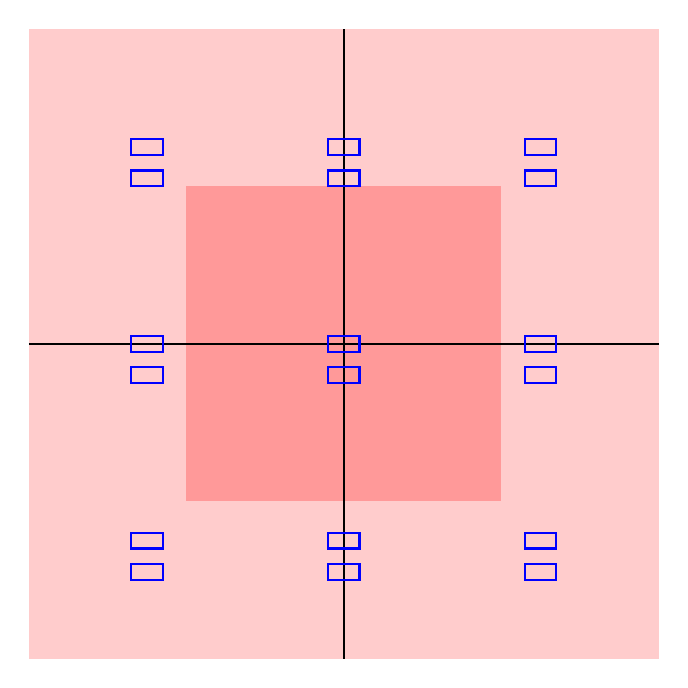
\begin{tikzpicture}
    % Parameters
    \def\coneHeight{3}
    \def\coneWidth{1}
    \def\rectWidth{0.4}
    \def\rectHeight{0.2}

    % Red cones (shaded area)
    \fill[red!20] (-4,0) -- (0,0) -- (0,-4) -- (-4,-4);
    \fill[red!20] (4,0) -- (0,0) -- (0,-4) -- (4,-4);
    \fill[red!20] (-4,0) -- (0,0) -- (0,4) -- (-4,4);
    \fill[red!20] (4,0) -- (0,0) -- (0,4) -- (4,4);

    % Red stronger cones
    \fill[red!40] (-2,0) -- (0,0) -- (0,-2) -- (-2,-2);
    \fill[red!40] (2,0) -- (0,0) -- (0,-2) -- (2,-2);
    \fill[red!40] (-2,0) -- (0,0) -- (0,2) -- (-2,2);
    \fill[red!40] (2,0) -- (0,0) -- (0,2) -- (2,2);

    % Axes
    \draw[thick] (-4,0) -- (4,0);
    \draw[thick] (0,-4) -- (0,4);

    % Blue rectangles
    \foreach \x in {-2.5, 0, 2.5} {
        \foreach \y in {-2.5, 0, 2.5} {
            \draw[blue, thick] (\x-0.2,\y-0.1) rectangle (\x+0.2,\y+0.1);
            \draw[blue, thick] (\x-0.2,\y-0.3) rectangle (\x+0.2,\y-0.5);
        }
    }

\end{tikzpicture}

\end{document}